\chapter{Metodología}\label{Metodología}
%Función que crea el título de capítulo y al cual se le da el nombre deseado a través de su parámetro obligatorio. Al no tener la función el “*” se escribirá también en el título del documento las palabras “Capítulo 1: …”. Además se indica, mediante la función “\label”, la correspondiente etiqueta que lleva asociada. La etiqueta sirve para que en caso de que luego se quiera hacer referencia al capítulo se haga llamando etiqueta tal que se escribiría “La información correspondiente a dicho tema se encuentra en el capítulo \ref{Int}.”

\thispagestyle{fancy}
%Función que determina que durante este capítulo se aplique el estilo Fancy.

\fancyhead[LE]{\thechapter.Metodología} 
%Función que se utiliza para indicar que en las páginas impares, aparezca en el encabezado en la parte izquierda, el número del capítulo con su correspondiente nombre.

\section{Desarrollo ágil}
Este proyecto nace de una idea tan amplia como el SSI. No había requisitos iniciales y ni se conocía el alcance. Para poder estudiar las posibilidades tan amplias con las que se puede afrontar se seleccionó la metodología SCRUM. Esta metodología se está pensada para equipos con reuniones periódicas. Cada sprint de trabajo tiene unos objetivos. Estos se comprobarán al final con una reunión.
En este caso, tras realizar un objetivo se aseguraba su funcionamiento y se comprobaba las metas. De este modo, podíamos asegurarnos de conseguir enfocar los requisitos del proyecto al mismo tiempo que asegurábamos el funcionamiento global de la aplicación.
Como SCRUM es una metodología extensa y complicada, por eso mismo, se va a introducir la metodología en este trabajo.
La metodología de trabajo SCRUM cuenta con cuatro pilares.
\begin{itemize}
    \item \textbf{Equipo SCRUM}\\
    Para poder realizar un trabajo, se necesita un motor para hacer mover las tareas. Ese motor es el equipo al que se le dan las tareas del sprint para realizar.
    En el caso de este proyecto, ha sido trabajo de solo una persona. Las reuniones de control se realizaban con el director del proyecto al final de cada sprint.
    \item \textbf{Backlog o lista de tareas}\\
    \begin{figure}[h!]
        \centering
        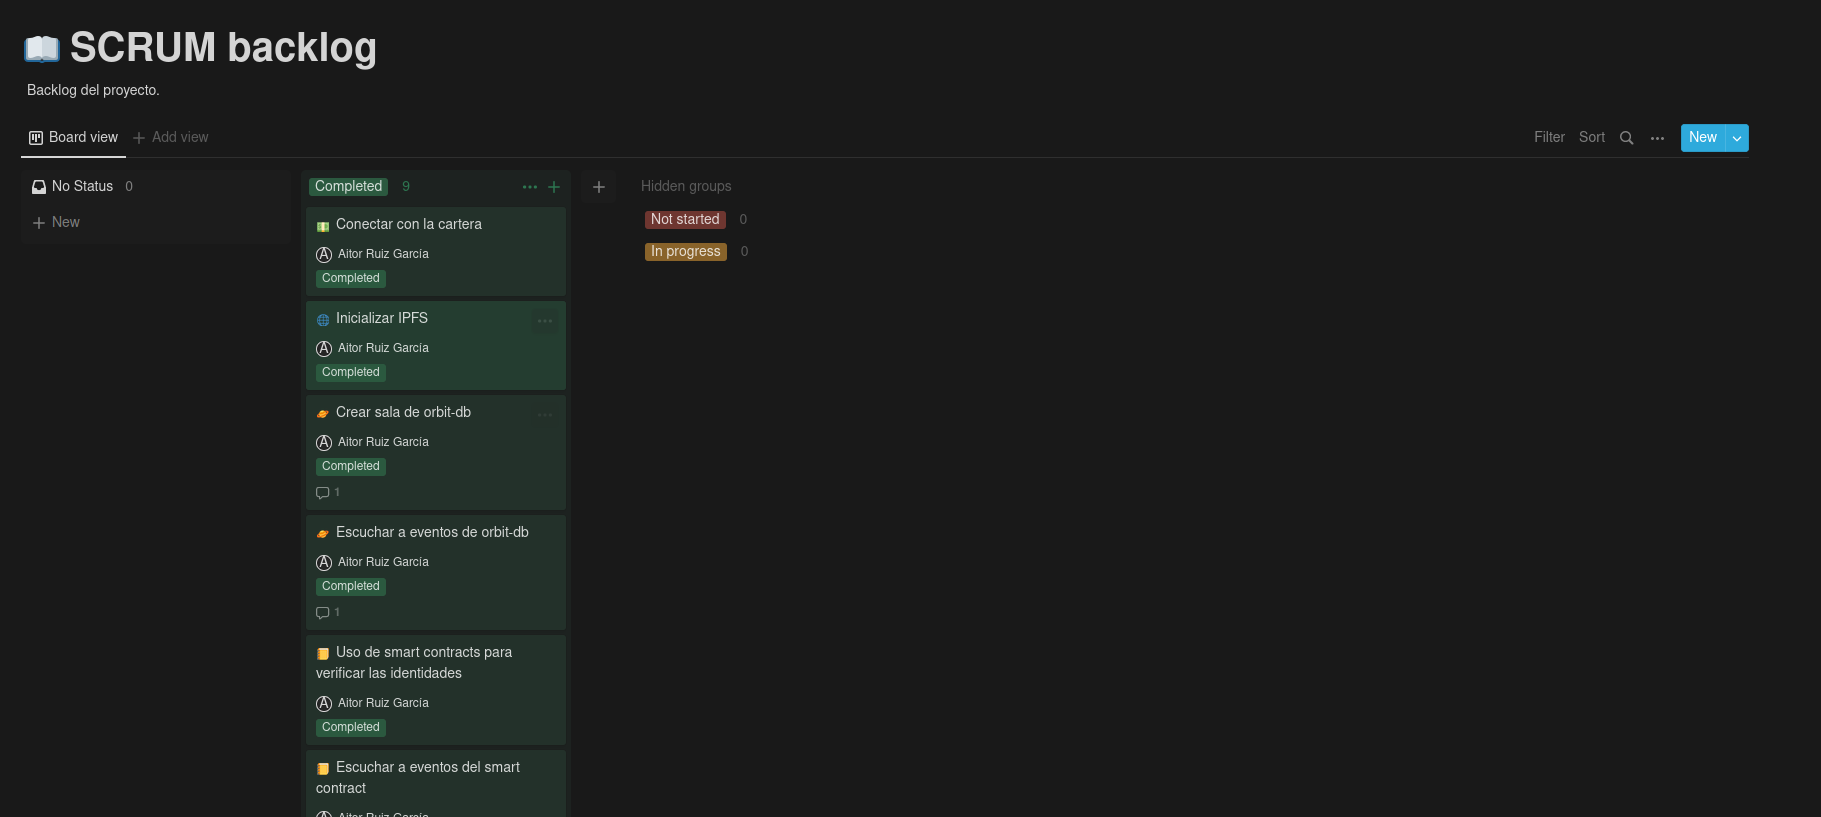
\includegraphics[width=0.8\textwidth]{Figures/Screenshot_20220601_182542.png}
        \caption{Imagen del backlog del proyecto}
        \label{fg:backlog}
    \end{figure}
    El desarrollo se ha estado controlando desde \verb|notion.so| \cite{web:notion}. Notion genera un archivo markdown. Este fichero puede ser enriquecido con distintos widgets. Uno de estos widgets es una board view.  Esta inspirado en otras herramientas que permiten hacer backlogs \ref{fg:backlog}.
    Se crearon temas que cumplían uno o varios requisitos del proyecto al mismo tiempo y que estaban relacionados entre si. Estas tarjetas pueden ser desplazadas dependiendo del estado en el que están.
    \begin{itemize}
        \item \verb|No iniciado|
        \item \verb|En proceso|
        \item \verb|Complatada|
    \end{itemize}
    Dentro de estas tarjetas se puede escribir y anotar elementos. Uno de los elementos importantes que se puede anotar son las horas invertidas en el desarrollo. Útil para las reuniones y para el presupuesto.
    \item \textbf{Sprint}\\
    Cuando se completa un sprint, si se ha completado la tarea correspondiente, la tarjeta deberá ser desplazada a completada.
    En esta tarjeta, si se selecciona, se puede acceder a la información en su interior \ref{fg:tarjeta}.
    \begin{figure}[h!]
        \centering
        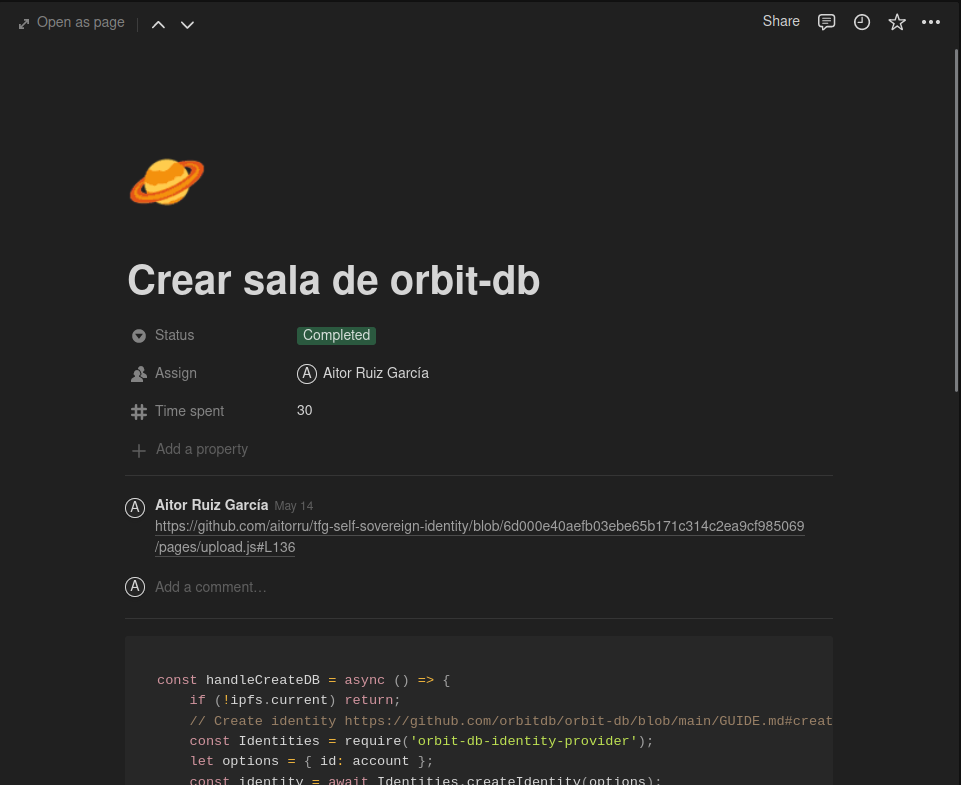
\includegraphics[width=0.7\textwidth]{Figures/Screenshot_20220601_181036.png}
        \caption{Imagen de los datos dentro de una tarjeta.}
        \label{fg:tarjeta}
    \end{figure}
    \item \textbf{Reuniones de seguimiento (bisemanales)}\\
    Para hacer las reuniones, se necesita tener un guion para hacer una revisión eficiente. Para poder apuntar información útil para la reunion, se usaba los comentarios asociados a la tarjeta. Ese conocimiento puede ser utilizado para el resto de los sprints.
\end{itemize}
\newpage
\section{Herramientas de desarrollo}
Un elemento fundamental para el desarrollo de esta aplicación, ha sido Nextjs. Es un framework para generar paginas estáticas, con capacidad de utilizar SSR (renderizado de servidor) y ISR (renderizado estático incremental).
En el apartado \textbf{Herramientas utilizadas}, se explicara el porque se ha elegido un framework basado en react.
Aun así, solo estamos interesados en dos aspectos.
\subsection{Paginas estáticas}
Como hemos dicho anteriormente, en IPFS \cite{web:ipfs} se pueden subir ficheros. Por lo cual podemos subir archivos \verb|.html|.
El esquema de acceso clásico en una pagina, todos los usuarios acceden a un servidor centralizado \ref{fg:centralizado}.
\begin{figure}[h!]
    \centering
    
\includegraphics[width=0.5\textwidth]{Figures/Centralizado.png}
    \caption{Imagen para explicar la centralización de un servidor. \textbf{El nodo con mayor tamaño es el servidor. El resto son usuarios que quieren conectarse.}}
    \label{fg:centralizado}
\end{figure}
Una implantation que cuente con mas recursos, puede tener mas nodos centralizados mas cerca de sus usuarios, pero eso solo se lo pueden permitir organizaciones con muchos recursos.
Cuando una pagina que no dispone de mas servidores repartidos por el mundo, solo tiene un punto de acceso. IPFS \cite{web:ipfs} viene al rescate ya que todos los ficheros que son compartidos, son cacheados. Haciendo que cuanto mas se use un fichero, mas fácil sea acceder a el.
Todos los ficheros estáticos pueden ser alojados en IPFS \cite{web:ipfs} y visitados de la siguiente manera. Tomando de ejemplo la documentación de IPFS \cite{web:ipfs} \cite{web:ipfs_whatis}, imaginemos que queremos acceder a Wikipedia \cite{web:wikipedia_main}.
El servidor de Wikipedia puede estar en un servidor al otro lado del mundo o en otro planeta. Aun así, en tu cercanía, seguro que otra persona más quiere acceder a Wikipedia. Para eso, podemos buscar si alguien tiene la pagina en la red de IPFS \cite{web:ipfs}.
\begin{quote}
    \verb|/ipfs/QmXoypizjW3WknFiJnKLwHCnL72vedxjQkDDP1mXWo6uco/wiki|
\end{quote}
Si introducimos este DID en el navegador, no significa nada, ya que de manera nativa no puede convertirse en un nodo de IPFS \cite{web:ipfs}. Por eso mismo, necesitamos una manera de ejecutar js-ipfs \cite{web:js-ipfs} (una librería que se explicará más adelante) para poder revivir el fichero.
Existen muchas puertas de entrada \ref{fg:ipfs_entry} e incluso se pueden crear nuevos.
\begin{figure}[h!]
    \centering
    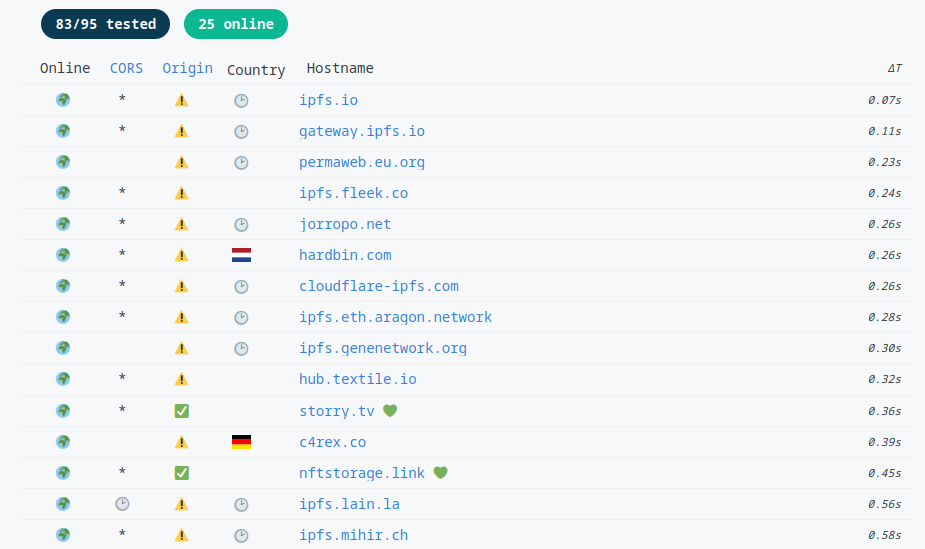
\includegraphics[width=0.7\textwidth]{Figures/ipfs_entry.png}
    \caption{Imagen de puntos de acceso de IPFS \cite{web:ipfs}}
    \label{fg:ipfs_entry}
\end{figure}
Por simplicidad vamos a utilizar el gateway de los creadores, \textbf{que no significa que sea oficial} eso no existe en el mundo distribuido.
\begin{quote}
    \url{https://ipfs.io/ipfs/QmXoypizjW3WknFiJnKLwHCnL72vedxjQkDDP1mXWo6uco/wiki/}
\end{quote}
De esta manera, tenemos acceso a una pagina de Wikipedia distribuida.
Esto también se puede aplicar al proyecto ya que de esta manera nextjs de manera predeterminada, solo exporta ficheros estáticos. Lo perfecto para IPFS \cite{web:ipfs}.
\subsection{Separación de código y empaquetado}
Todas las librerías de web 3.0, están en un estado muy temprano y por ende no están optimizadas para ocupar poco espacio. Aunque nuestra pagina puede estar alojada en IPFS \cite{web:ipfs} y resulte en tiempos de respuestas mas bajos, no significa que no haya que optimizar el tiempo de descarga del bundle de js.
Para comprender mejor el problema y como poder aliviarlo, vamos a poner un ejemplo.
Next.js \cite{web:next.js}, aunque exporta HTML estático, es un framework que utiliza react para construir la interfaz. Mas adelante, se explicará que es react y porque esta seleccionado para este proyecto. Por ahora solo hay que saber que es un archivo de js que nuestro navegador tiene que ejecutar para que nuestra pagina pueda hacer algo útil.
En JavaScript, hay dos maneras de importar funcionalidad en un proyecto.\\
\textbf{Require}\\
\begin{lstlisting}
    // Este codigo no es recomendable.
    const react = require('react');
\end{lstlisting}
\noindent\rule{\textwidth}{0.4pt}
\textbf{Modules}\\
\begin{lstlisting}
    import react from 'react';
\end{lstlisting}
La diferencia principal es que require es síncrono e import es asíncrono.
Esto quiere decir que si es síncrono, cada instrucción se ejecuta una detrás de la anterior. En cambio con import, se deja cargando y se pasa a la siguiente instrucción.
Aunque los módulos están gradualmente adoptados \cite{web:canIuse}, han sido añadidos al \textit{spec} \cite{web:ecma}. A fecha de creación de este proyecto, Next.js \cite{web:next.js} esta configurado para hacer todo su código compatible con EC6. El spec a fecha de 2015.
\begin{quote}
    Next.js \cite{web:next.js} supports \textbf{IE11 and all modern browsers} (Edge, Firefox, Chrome, Safari, Opera, et al) with no required configuration. \cite{web:next_supported}
\end{quote}
\begin{center}
    \begin{table}[h!]
        \begin{tabular}{p{0.3\linewidth}  p{0.6\linewidth}}
                \verb|import react from 'react';|
            & 
\verb|use strict';|

\verb|var _react = require('react');|
             \\
            Como vemos, nuestro import compacto y asíncrono en el spec de 2015, se convierte en un conjunto de código síncrono y extenso. & 
\verb|var _react2 = _interopRequireDefault(_react);|

\verb|function _interopRequireDefault(obj)|
\verb|{ return obj && obj.__esModule ? obj : { default: obj }; }|

\\
        \end{tabular}
        \label{tab:EC6_output}
        \caption{Tabla explicando el desglose de un mensaje de ethereum.}
    \end{table}
\end{center}
Esto es malo para el rendimiento ya que si tenemos muchos \verb|require| nuestra pagina tardará mas en ser interactiva porque está esperando a que el resto de módulos se lleguen a descargar y verificar.
Por eso mismo, Next.js \cite{web:next.js} nos permite hacer lo siguiente.
\begin{lstlisting}
    // ...
    async function foo() {
        // Libreria de ejemplo
        const Fuse = (await import('fuse.js')).default
    }
    // ...
\end{lstlisting}
Cuando se ejecute la function \verb|foo|, se descargará y validará en ese momento. Delegando el peso de descargar las librerías necesarias cuando se van a usar hace que nuestra pagina sea interactiva más rápido.
\subsection{Remix}
Remix es un entorno de desarrollo integrado para poder desarrollar smart contracts. Dispone de una red de prueba, a demás de ser capaz de comunicarse con la cartera. De esta manera podemos hacer todas las prueba que queramos sin tener que quemar gas por el camino. Entiéndase gas como traducción directa de quemar dinero.
Ya que nuestro entrono de desarrollo local, tiene una implementación local utilizando ganache, que se menciona mas adelante, estamos interesados en utilizar metamask para conectarnos directamente a la red de prueba \ref{fg:remix}.
\begin{figure}[h!]
    \centering
    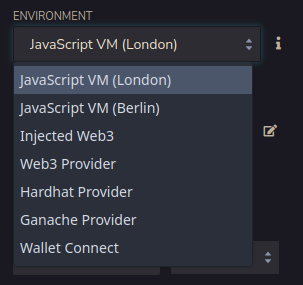
\includegraphics[width=0.4\textwidth]{Figures/remix.png}
    \caption{Posibles conexiones de Remix.}
    \label{fg:remix}
\end{figure}
Metamask, de manera predeterminada se conectara a la red principar de Ethereum e integrará una variable especial en el objeto \verb|window| de nuestro navegador.
\begin{lstlisting}
    if (typeof window.ethereum !== 'undefined') {
        console.log('MetaMask is installed!');
    }
\end{lstlisting}
De la siguiente manera, podemos comprobar si metamask esta instalado.
Como desarrollador, solamente tienes que seleccionar una dirección local para empezar.
\subsection{Ganache}
Ganache permite generar redes blockchain locales. Metamask se puede conectar a esta red e interactuar con ella.
\begin{lstlisting}
    ganache-cli -p 8545 --mnemonic 
    \" word desert grief seven feature sight 
    object message upon lesson boat praise \" 
    --networkId 1337 --db ganache/db -q
\end{lstlisting}
Con el siguiente comando, podemos establecer un puerto con \verb|-p 8545|, asegurarnos de cargar las mismas cuentas estableciendo un nemotecnico, establecer el id de la red, la cual tiene que ser 1337 ya que es local y por ultimo, establecer una ruta para guardar todos los datos de la red. Es decir todos los bloques.
\subsection{Control de versiones}
Para este proyecto, se ha seleccionado git como aplicación de control de versiones y GitHub \ref{fg:github} como repositorio remoto. Como este proyecto usa y es código abierto, se ha usado un repositorio publico para poder mostrar todos los pasos de desarrollo. De esa manera queda expuesto todos los commits asociados a sprints.
Este repositorio también es útil como expositor temporal. Cualquier persona puede ver el desarrollo y verificar la integridad de nuestra solución.
\begin{figure}
    \centering
    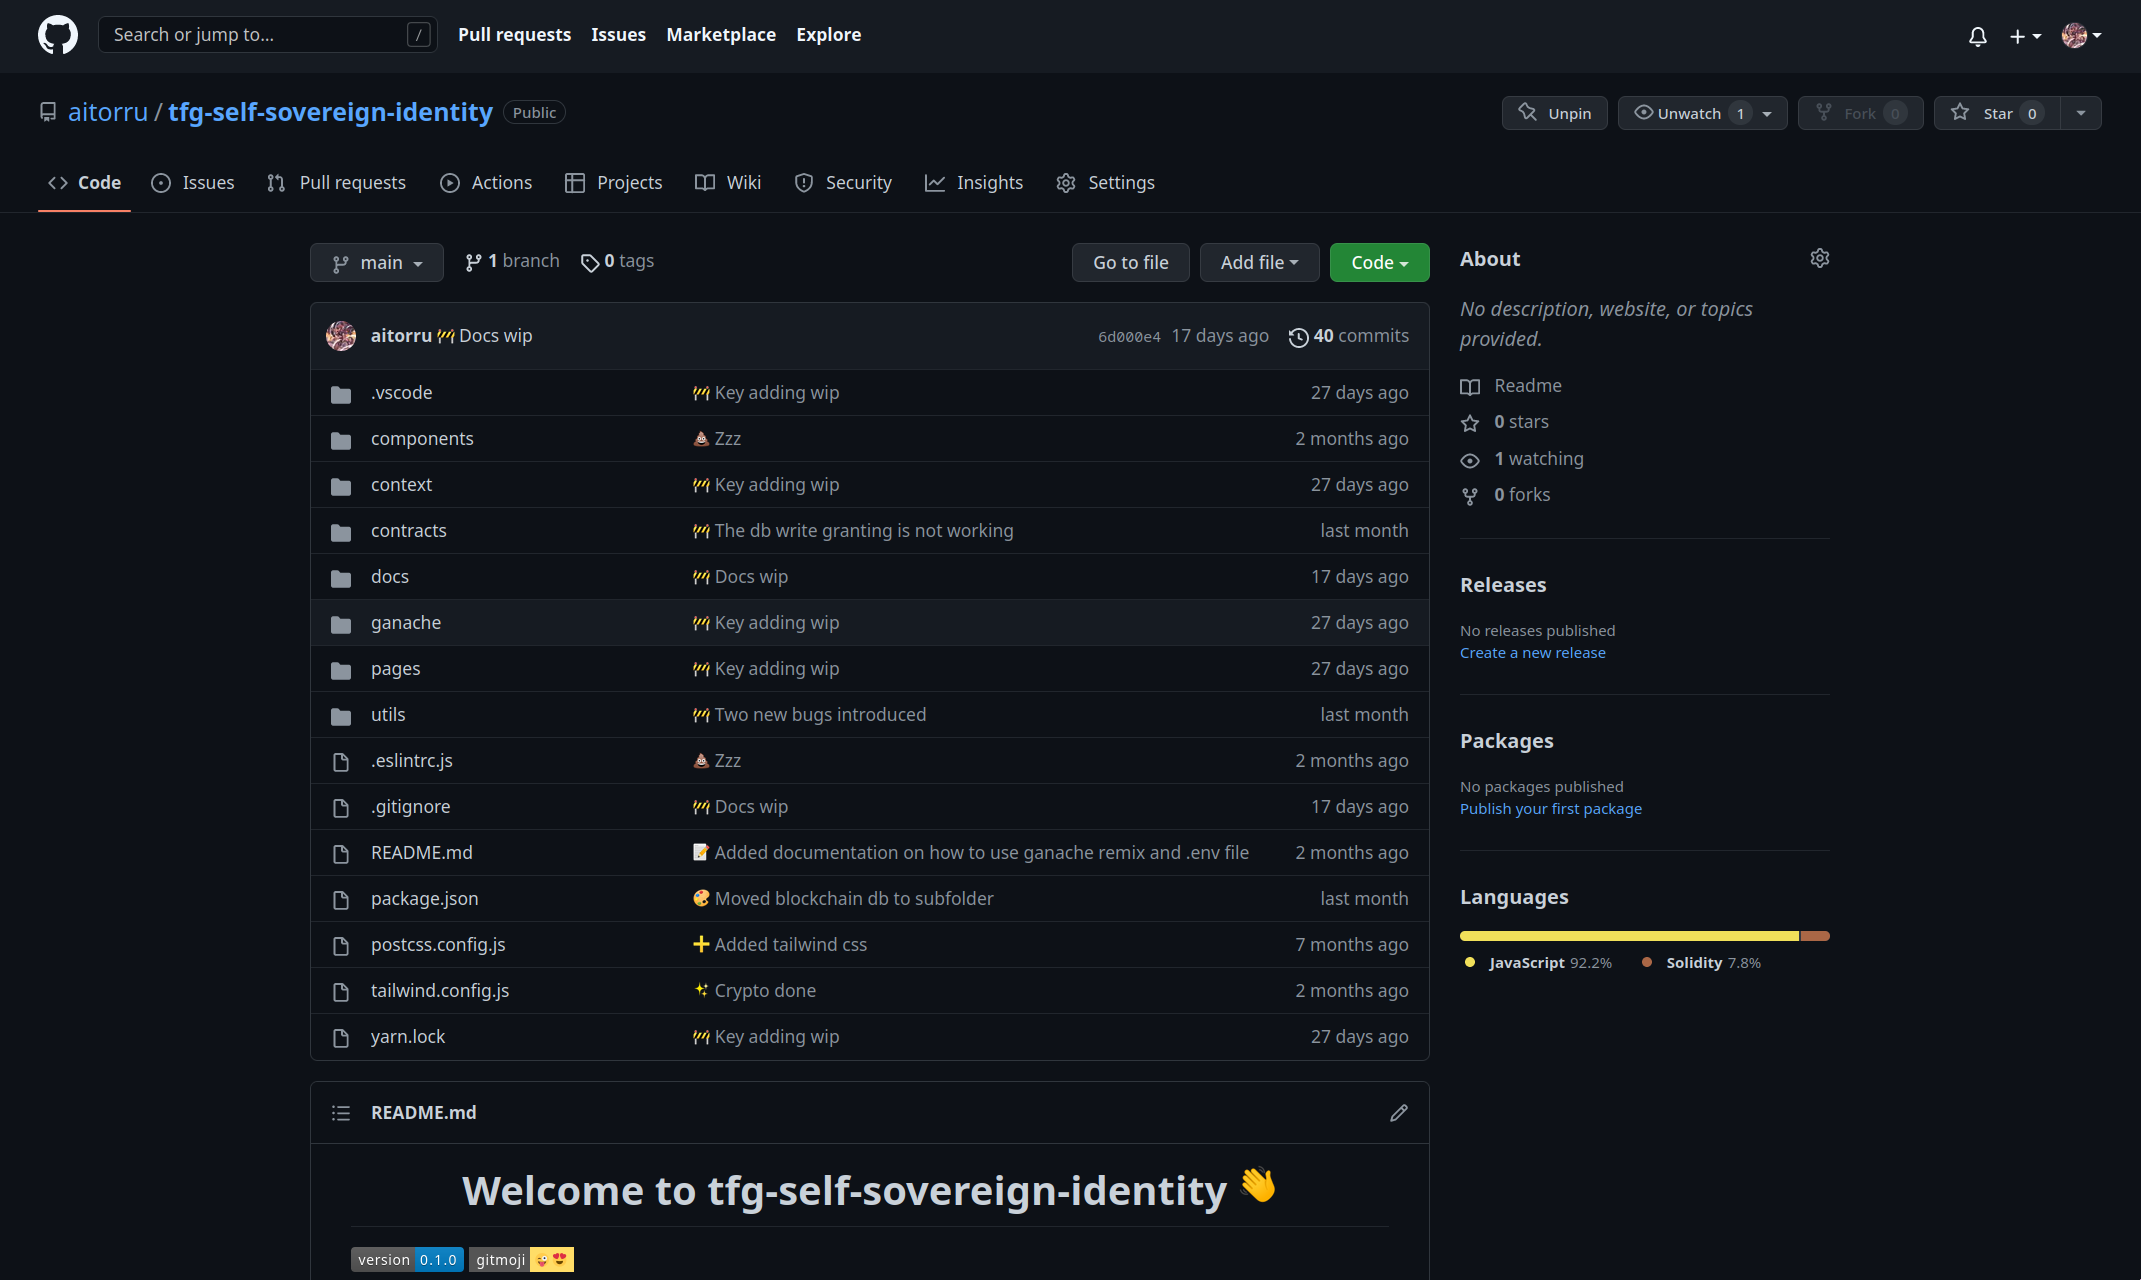
\includegraphics[width=0.5\textwidth]{Figures/github.png}
    \caption{Repositorio de github del proyecto}
    \label{fg:github}
    \cite{web:repo}
\end{figure}
\subsection{Contexto}
Para una planificación de temas, se usó una herramienta diferente. En vez de utilizar un fichero o una nota en notion.so, se decidió utilizar apuntes en el código. Como se tenia acceso a los objetivos desde el inicio del desarrollo, se podían crear funciones vacías a modo de punto de inicio. Después se pueden crear comentarios para generar contexto.
\begin{lstlisting}
    // TODO: Hacer funcionar el proyecto
    // FIXME: El reloj no devuelve el tiempo en ISO
\end{lstlisting}
Todos los IDEs, tienen la capacidad de generar arboles de \verb|TODOs| y \verb|FIXMEs|. En Code - OSS \cite{web:code-oss}, un clon de código abierto de vscode, existen extensiones para facilitar el proyecto.
De esta manera, los comentarios \ref{fg:todoTree} nos sirven como herramienta de contexto a lo largo de un sprint.
\begin{figure}[h!]
    \centering
    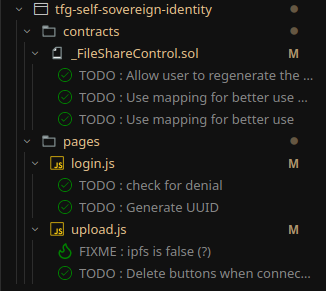
\includegraphics[width=0.5\textwidth]{Figures/TodoTree.png}
    \caption{Ejemplo de visualización de comentarios}
    \label{fg:todoTree}
\end{figure}
\newpage
\thispagestyle{empty}